% Volume III chapter: Wiener covariance, Riesz means and the positive Maslanka criterion. Sources: misc/reviews/nick-chebyshev-wiener/chebyshev_wiener_chapter_for_vadim/chebyshev_wiener_chapter.tex lines 97 to 99, 291 to 536 (Sections 1 to 7 and 12 reduced to cross references); referee misc/research/directions/opus/vol3/CW.md (M1 to M10, overlap recommendation); numbers misc/vol3/verify/CW/results.md; 17 Nov 2026 brief with the 7/8 half plane read as a theorem (misc/vol3/QRH78_DECISION.md).
% Coordinator notes: label prefix cw:; new bibliography file ch/nc_v3_cw_bib.tex (DunlopNewman75, UNCHECKED, to be pooled). Keys used from ch/bib.tex: Cramer, Lagarias, Garunkstis02, Salem53, Wiener32, LVJ, Williamson, BaezDuarte03, BaezDuarte10, Maslanka01, Grigelionis99, PSW13, OAI26a, BNKS82; RubinsteinSarnak94 is in ch/nc_v3_bond2_bib.tex. Figures fig/v3/cw_maslanka.pdf and fig/v3/cw_maslanka_sin2.pdf (Figures 3 and 4 of the note; the verification confirmed every number quoted in their captions and Tables 3 and 4, but did not regenerate the plots). Figures 1 and 2 of the note are dropped: Figure 1 quotes errors that the recomputation did not reproduce. The positive Maslanka criterion is cw:thm:maslanka, the Williamson tilted densities are cw:prop:williamson. MH chapter: its restatement of T_k and the pole against zero argument may now cite cw:prop:williamson, and its atoms r_j=gamma_j^2/2 are in the note's chart (twice too small in the book's chart).
\label{cw:ch:wiener}

This chapter records what a note on Chebyshev's error and Wiener's spectrum adds to the chapter on Chebyshev's memoirs (Chapter~\ref{ct:ch:cheb}). Results are from an unrefereed note of Polson (November 2026) unless a source is named. We use the book's chart: the Laplace variable is $u=w^2$, the Thorin variable is $z=r^2$, and the centre atoms are $\gamma^2$. The note works in the chart $u=w^2/2$, so every rate below is twice the note's. The symbol $\xi$ is Riemann's, with the factor $\frac12s(s-1)$, and $G=\xi'/\xi$. As in Chapter~\ref{ct:ch:cheb}, $v_\alpha(r)=\Re G(\alpha+ir)$, $b_\alpha=G(\alpha)$ and $t_\alpha(z)=(v_\alpha(r)-b_\alpha)/(2\pi r)$ with $r=\sqrt z$. Status words follow the book: proved, computed (floating point), certified (ball arithmetic), conditional, heuristic, open.

\section{What the note repeats}\label{cw:sec:known}

Most of the note is in the book already, and we cite it instead of reprinting it. Chebyshev's identity with exponential weights and the three kernels (Bose, Fermi Dirac, hyperbolic secant) are the inversion of Lai and Vere-Jones (Proposition~\ref{rz:prop:lvj}, \cite{LVJ}) and the eta combination of Section~\ref{ct:sec:strip}. Riesz's and Hardy and Littlewood's criteria are in Chapter~\ref{ch:riesz}. Wiener's closure theorem, Salem's kernel and Kac's proof are in Sections~\ref{wr:sec:wiener}, \ref{wr:sec:salem} and \ref{lv:sec:salem} (\cite{Wiener32}, \cite{Salem53}). The Poisson form of the Thorin density, the Landau converse and the effect of an off line zero are Theorem~\ref{thm:poisson} and Proposition~\ref{prop:struct}, and in the Chebyshev language Theorem~\ref{ct:thm:dictionary} and Lemma~\ref{ct:lem:onepair}. The error form is Theorem~\ref{ct:thm:budget}, with $\mathcal T_\alpha[E]=-\mathrm{Osc}_\alpha$ and its continuation below level one in Proposition~\ref{ct:prop:levy}. The level criterion is Proposition~\ref{ct:prop:qrh}, Theorem~\ref{thm:dbeta:minall} and Lagarias \cite{Lagarias}, and the small $q$ behaviour of $v_\alpha-b_\alpha$ is the curvature of Proposition~\ref{ct:prop:curv}. Rung one is Proposition~\ref{bp:prop:valpha} in ball arithmetic and Section~\ref{ct:sec:rung}, after Garunk\v{s}tis \cite{Garunkstis02}. The note's own proof of that rung used a floating point step and a bound on $S(T)$ that does not reach height $2000$ in the form needed, so we do not repeat it.

Every rung $\alpha>\frac78$ is a theorem: by the theorem of \cite{OAI26a} the function $\xi$ has no zero in $\Re s>\frac78$, and Proposition~\ref{ct:prop:qrh} turns that into $t_\alpha\ge0$. The first open rung is $\alpha=\frac78$, and RH is the step from $\frac78$ to $\frac12$. The path through the ladder, and why the missing step is the Cauchy deconvolution, is Section~\ref{ct:sec:path}.

\begin{remark}[the logistic law]\label{cw:rem:logistic}
Wiener's closure theorem detects zeros of a transform and does not use positivity, while Landau's theorem is one sided. The link is the logistic law. Salem's kernel is the logistic survival function, $1/(e^v+1)=\int_v^\infty\frac14\mathrm{sech}^2(t/2)\,\dd t$. The logistic density is a $z$ distribution of Barndorff-Nielsen, Kent and S\o rensen \cite{BNKS82} with characteristic function $\pi t/\sinh\pi t=\prod_{k\ge1}(1+t^2/k^2)^{-1}$, a generalised gamma convolution in $t^2$ with Thorin atoms $k^2$. So the kernel of Salem's criterion is a Thorin object in the additive variable $v$, while the criterion lives in the Mellin variable. We do not know how to transport the positivity from one to the other (open).
\end{remark}

\section{The Stieltjes transform is a Wiener cross covariance}\label{cw:sec:cov}

For real $a\notin\{\frac52,\frac92,\frac{13}2,\dots\}$ let $\kappa=\frac12-a$ and define the weighted Chebyshev error
\[
E_a(y)=e^{-ay}\Big[\sum_{n\le e^y}\frac{\Lambda(n)}{n^{\kappa}}-\frac{e^{(1-\kappa)y}}{1-\kappa}+\frac{\zeta'}{\zeta}(\kappa)\Big],
\]
with the bracket read as $\sum_{n\le x}\Lambda(n)/n-\log x+\gamma$ when $\kappa=1$. Thus $E_{1/2}$ differs by $o(1)$ from Chebyshev's error $(\psi(x)-x)/\sqrt x$ and $E_{-1/2}$ is the Mertens error $\sqrt x\,(\sum_{n\le x}\Lambda(n)/n-\log x+\gamma)$. Assume RH and simple zeros. Then the explicit formula gives $E_a(y)=-\sum_\gamma e^{i\gamma y}/(a+i\gamma)+o(1)$ in mean square, the sum over the ordinates of both signs.

\begin{theorem}[covariance identity]\label{cw:thm:cov}
(i) For every $\alpha>\Theta=\sup\Re\rho$, and so by the theorem of \cite{OAI26a} for every $\alpha>\frac78$, and for every $w>0$,
\[
\int_0^\infty\frac{t_\alpha(z)\,\dd z}{z+w^2}=\frac{G(\alpha+w)-G(\alpha)}{2w}.
\]
(ii) Assume RH and simple zeros. For such $a,a'$ with $a+a'\ne0$ the mean square covariance
\[
\begin{aligned}\mathrm{Cov}(E_a,E_{a'})&=\lim_{Y\to\infty}\frac1Y\int_0^YE_a(y)E_{a'}(y)\,\dd y\\&=\sum_\gamma\frac1{(a+i\gamma)(a'-i\gamma)}=\frac{G(\frac12+a)+G(\frac12+a')}{a+a'},\end{aligned}
\]
and $\mathrm{Var}\,E_a=G(\frac12+|a|)/|a|$ for $a\ne0$. For $a+a'=0$ the covariance is $G'(\frac12+|a|)$. In particular, with $a=\alpha-\frac12+w$ and $a'=\frac12-\alpha$ the covariance of the errors of $\sum_{n\le x}\Lambda(n)n^{-\alpha}$ and $\sum_{n\le x}\Lambda(n)n^{\alpha+w-1}$ is $(G(\alpha+w)-G(\alpha))/w$, twice the Stieltjes transform in (i).
\end{theorem}

\begin{proof}
(i) The function $w\mapsto G(\alpha+w)$ is analytic in $\Re w>0$ when $\alpha>\Theta$, and its real part is $O_\alpha(\log(2+|w|))$. A harmonic function of that growth is the Poisson integral of its boundary values. Using $\Re G(\alpha-ir)=\Re G(\alpha+ir)$ and $\frac2\pi\int_0^\infty\frac{w\,\dd q}{w^2+q^2}=1$ gives $G(\alpha+w)-G(\alpha)=\frac1\pi\int_0^\infty\frac{2w}{w^2+r^2}(v_\alpha(r)-b_\alpha)\,\dd r$. Put $z=r^2$, so that $\dd z=2r\,\dd r$ and $t_\alpha(z)\,\dd z=(v_\alpha(r)-b_\alpha)\,\dd r/\pi$.
(ii) The mean of $e^{i(\gamma-\gamma')y}$ vanishes unless $\gamma=\gamma'$, which gives the sum. Next, $\frac1{(a+i\gamma)(a'-i\gamma)}=\frac1{a+a'}\big[\frac1{a+i\gamma}+\frac1{a'-i\gamma}\big]$, and $\sum_\gamma\frac1{a+i\gamma}=G(\frac12+a)$ by the Hadamard product, with $G(1-s)=-G(s)$. At $a'=-a$ the sum is $-\sum_\gamma(a+i\gamma)^{-2}=G'(\frac12+a)$.
\end{proof}

Simple zeros are needed in (ii). A zero of multiplicity $m$ enters the mean square with weight $m^2$, while $\sum_\gamma1/(a+i\gamma)=G(\frac12+a)$ counts it $m$ times. Linear independence of the ordinates is not needed for second moments. For $\alpha>1$ no hypothesis on zeros is used in (i). At the centre, $a=\frac12$ gives $\mathrm{Var}\,E_{1/2}=2G(1)=2+\gamma-\log4\pi=0.046191$, the variance identity of Remark~\ref{ct:rem:cramer} (Cram\'er \cite{Cramer}). With $a'=-a=-\frac12$ the covariance of the Chebyshev and Mertens errors is $G'(1)=0.046154$. At $a=\frac12$, $a'=0$ the value $\mathrm{Cov}(E_{1/2},E_0)$ equals $\mathrm{Var}\,E_{1/2}$ only because $G(\frac12)=0$.

In Wiener's terms the spectral measure of $E_a$ is $\sum_\gamma\delta_\gamma/(a^2+\gamma^2)$. In the Thorin variable it is the centre measure $U_{\rm RH}=\sum_{\gamma>0}\delta_{\gamma^2}$, weighted by the Stieltjes kernel $2/(z+a^2)$. General weighted covariances are not in Cram\'er's centre variance and are not in Chapter~\ref{ct:ch:cheb}. They are classical mean value theorems for explicit formula sums, and the Stieltjes reading is the new point.

\begin{table}[t]
\centering\small
\begin{tabular}{lrr}
\toprule
Quantity & Predicted & Primes to $10^7$\\
\midrule
$\mathrm{Var}\,E_{1/2}$ (Chebyshev) & 0.046191 & 0.046747\\
$\mathrm{Var}\,E_{1/4}$ & 0.046205 & 0.046760\\
$\mathrm{Var}\,E_{-1/4}$ & 0.046205 & 0.046759\\
$\mathrm{Var}\,E_{-1/2}$ (Mertens) & 0.046191 & 0.046744\\
$\mathrm{Cov}(E_{-1/2},E_{1/2})$ & 0.046154 & 0.046709\\
$\mathrm{Cov}(E_{-1/4},E_{1/4})$ & 0.046196 & 0.046750\\
$\mathrm{Cov}(E_{-1/4},E_{1/2})$ & 0.046177 & 0.046732\\
Riesz mean $k=1$, Proposition~\ref{cw:prop:riesz} & $7.363\times10^{-5}$ & $7.396\times10^{-5}$\\
\bottomrule
\end{tabular}
\caption{Theorem~\ref{cw:thm:cov} against the primes (computed). The sieve covers the $665\,134$ prime powers up to $10^7$, with $200\,000$ points equally spaced in $y=\log x$ with $x$ in $[10^3,10^7]$ and the mean product removed. The Riesz row includes the constant term of the explicit formula. The predicted column was recomputed to the digits shown, with $34$ digit arithmetic.}
\label{cw:tab:cov}
\end{table}

Table~\ref{cw:tab:cov} compares the two sides. They agree within $1.2$ percent, and the ordering of the three covariances is reproduced. The rows differ little because the first zero is high. The point is that the prime side reproduces the Thorin side at every level, with the same finite sample bias of about $5.5\times10^{-4}$.

\begin{remark}[the prime side of the budget form]\label{cw:rem:primes}
Theorem~\ref{ct:thm:budget} can be evaluated from primes alone. Take the second form of the error transform, with the exact $E(y)$ for $e^y\le10^7$, integrated piece by piece. At $\alpha=\frac32$ the maximal error against $v_\alpha-b_\alpha$ on $0<q\le120$ is of the order $10^{-7}$ (computed). At $\alpha=1$ it is $7\times10^{-4}$ for $q\le40$ and grows with the range of $q$. At $\alpha=\frac34$ (a comparison that tests the identity only if $\Theta<\frac34$, so it is conditional) it is $0.07$ for $q\le40$, because truncation at $10^7$ leaves a factor $e^{-by}=0.018$ at $b=\frac14$. We print no minimum of the total near $q=0$: there $v_\alpha-b_\alpha$ is of order $q^2$ (Proposition~\ref{ct:prop:curv}), so any value on a grid starting at $q_0>0$ measures $q_0$ and not the density.
\end{remark}

\section{Riesz means are Williamson mixtures}\label{cw:sec:riesz}

Williamson \cite{Williamson} showed that a function on $(0,\infty)$ is $k$ monotone if and only if it is a scale mixture of the kernels $(1-t/x)_+^{k-1}$. As $k\to\infty$ these become exponentials and the statement becomes Bernstein's theorem. On the prime side the Williamson kernels are the typical means of Marcel Riesz,
\[
\psi_k(x)=\sum_{n\le x}\Lambda(n)\Big(1-\frac nx\Big)^k=\frac{x}{k+1}-\sum_\rho\frac{k!\,x^\rho}{\rho(\rho+1)\cdots(\rho+k)}+O(1).
\]
So $t\mapsto\psi_k(1/t)=\sum_n\Lambda(n)(1-nt)_+^k$ is the Williamson mixture of order $k+1$ with mixing measure $\sum_n\Lambda(n)\delta_{1/n}$. Chebyshev's $\psi$ is the case $k=0$, and the Abel sum $\sum\Lambda(n)e^{-nt}$ is the limit $k\to\infty$ with $x=k/t$. The typical means are classical (Riesz); the Williamson naming is from the note. They differ from the Williamson measures of the clock in Section~\ref{sec:ch12:kmono}, which are attached to $\xi$ and not to the primes.

\begin{proposition}[Riesz means]\label{cw:prop:riesz}
Assume RH and simple zeros. The normalised error $(\psi_k(x)-x/(k+1))/\sqrt x$ has spectral masses $k!^2\prod_{j=0}^k\big((j+\frac12)^2+\gamma^2\big)^{-1}$ at the ordinates $\pm\gamma$. Its variance is the finite combination
\[
\sum_{j=0}^k\frac{c_j\,G(j+1)}{j+\frac12},\qquad c_j=\frac{k!^2}{\prod_{i\ne j}\big((i+\frac12)^2-(j+\frac12)^2\big)},
\]
the $c_j$ being the partial fraction coefficients of the spectral mass. For $k=1$,
\[
\mathrm{Var}=\sum_\gamma\frac{1}{(\frac14+\gamma^2)(\frac94+\gamma^2)}=G(1)-\tfrac13G(2)=7.363\times10^{-5}.
\]
If in addition the ordinates are linearly independent over $\mathbb Q$, the limiting law has moment generating function $\prod_{\gamma>0}I_0(a_\gamma u)$ with $a_\gamma=2k!\big/\prod_{j=0}^k\sqrt{(j+\frac12)^2+\gamma^2}$, and the reciprocal is a generalised gamma convolution in $u^2$ with Thorin atoms $j_m^2\prod_{j=0}^k\big((j+\frac12)^2+\gamma^2\big)/(4\,k!^2)$, where $j_m$ are the positive zeros of $J_0$.
\end{proposition}

\begin{proof}
Divide the explicit formula by $\sqrt x$ and use the argument of Theorem~\ref{cw:thm:cov}(ii): the coefficient of $x^{i\gamma}$ is $k!/\prod_j(\rho+j)$ with $|\rho+j|^2=(j+\frac12)^2+\gamma^2$. Partial fractions in $\gamma^2$ give $k!^2/\prod_j((j+\frac12)^2+\gamma^2)=\sum_jc_j/((j+\frac12)^2+\gamma^2)$ with $c_j=k!^2/\prod_{i\ne j}((i+\frac12)^2-(j+\frac12)^2)$, and $\sum_\gamma1/(\lambda^2+\gamma^2)=G(\frac12+\lambda)/\lambda$ by Theorem~\ref{cw:thm:cov}(ii). For $k=1$, $c_0=\frac12$ and $c_1=-\frac12$. For the law, use independent uniform phases and $1/I_0(x)=\prod_m(1+x^2/j_m^2)^{-1}$.
\end{proof}

The sum over $8000$ zeros gives $7.3631788\times10^{-5}$ against $G(1)-G(2)/3=7.3631789\times10^{-5}$ (computed), and the primes give $7.396\times10^{-5}$ (Table~\ref{cw:tab:cov}). Williamson smoothing of order $k$ acts on the Thorin measure by a polynomial change of variable in $\gamma^2$: going from order $k-1$ to $k$ multiplies the atom by $((k+\frac12)^2+\gamma^2)/k^2$.

\begin{remark}
There is no $2\sin^2$ lemma for a single Williamson kernel of finite order on the $w$ side. For fixed $x>0$ the function $(1-wx/k)_+^k+wx-1$ is not real analytic at $w=k/x$, while a drift $cw^2$ plus a mixture of $\log(1+w^2/z)$ is real analytic in $w>0$. For single kernels positivity transfers to Thorin measures only at the exponential end $k=\infty$; special mixtures are not excluded. Williamson kernels belong on the prime side, as smoothers of the L\'evy measure, where they make the explicit formula absolutely convergent for $k\ge1$.
\end{remark}

\section{A positive Ma\'slanka criterion}\label{cw:sec:maslanka}

Ma\'slanka \cite{Maslanka01} expanded $(s-1)\zeta(s)$ in Pochhammer polynomials of $s/2$ (Proposition~\ref{prop:ch19:maslanka}), and B\'aez-Duarte \cite{BaezDuarte03,BaezDuarte10} deduced a discrete form of Riesz's criterion: RH holds if and only if $c_k=\sum_{j}(-1)^j\binom kj/\zeta(2j+2)=O(k^{-3/4+\varepsilon})$. Summing the binomial, $c_k=\sum_n\mu(n)n^{-2}(1-n^{-2})^k$, a Hausdorff moment sequence in $k$ at the points $t=n^{-2}$ with the signed M\"obius measure, whose exponential limit is Riesz's function. Replace $1/\zeta$ by $-\zeta'/\zeta$ and the mixing measure becomes positive. Let
\[
d_k=\sum_{j=0}^k(-1)^j\binom kj\Big(-\frac{\zeta'}{\zeta}\Big)(2j+2)=\sum_{n\ge2}\frac{\Lambda(n)}{n^2}\Big(1-\frac1{n^2}\Big)^k .
\]

\begin{theorem}[positive Ma\'slanka criterion]\label{cw:thm:maslanka}
(i) $d_k=\int_0^1(1-t)^k\nu(\dd t)$ with $\nu=\sum_n\Lambda(n)n^{-2}\delta_{n^{-2}}\ge0$, so $(d_k)$ is a completely monotone sequence: with $\Delta d_k=d_{k+1}-d_k$, $(-1)^r\Delta^rd_k=\int_0^1t^r(1-t)^k\nu(\dd t)\ge0$ for all $r,k\ge0$.

(ii) For $\Re z<\frac12$, $\;-\frac{\zeta'}{\zeta}(2-2z)=\sum_{k\ge0}d_k\,\frac{(z)_k}{k!}$, where $(z)_k$ is the Pochhammer symbol.

(iii) For $k\ge1$, with $B$ the Beta function,
\[
d_k=\tfrac12B\big(\tfrac12,k+1\big)-\frac{1}{2k(k+1)}-\tfrac12\sum_\rho B\big(1-\tfrac\rho2,k+1\big),
\]
and $R_k:=d_k-\tfrac12B(\tfrac12,k+1)=\int_1^\infty x^{-2}(1-x^{-2})^k\,\dd\Delta(x)$ with $\Delta(x)=\psi(x)-x$, the Williamson transform of the Chebyshev error.

(iv) RH holds if and only if $R_k=O(k^{-3/4+\varepsilon})$ for every $\varepsilon>0$. Under RH, $R_k=O(k^{-3/4})$. In general $R_k=O(k^{-1+\Theta/2})$, so by the theorem of \cite{OAI26a} one has $R_k=O(k^{-9/16})$ (proved).
\end{theorem}

\begin{proof}
(i) is the definition. (ii) For $0<t<1$, $t^{-z}=\sum_k(z)_k(1-t)^k/k!$. Integrate against $\nu$, with Fubini for real $0<z<\frac12$ and analytic continuation in $z$. (iii) The Mellin transform of $(1-t)_+^k$ is $B(z,k+1)$, so $d_k=\frac1{2\pi i}\int_{(c)}B(z,k+1)\big(-\frac{\zeta'}{\zeta}\big)(2-2z)\,\dd z$ for $0<c<\frac12$. Move the contour to the right. The pole of $\zeta$ gives $\frac12B(\frac12,k+1)$, a zero $\rho$ gives $-\frac12B(1-\frac\rho2,k+1)$, and the trivial zeros give $-\frac12\sum_{m\ge1}B(1+m,k+1)=-\frac12B(2,k)=-1/(2k(k+1))$. Since $B(z,k+1)=k!/\prod_{j=0}^k(z+j)$ decays like $|z|^{-k-1}$, the arcs vanish for $k\ge1$. Also $\int_1^\infty x^{-2}(1-x^{-2})^k\,\dd x=\frac12B(\frac12,k+1)$, which gives the error form. (iv) With $x=\Re z=1-\beta/2$, $|B(z,k+1)|\le\frac1{|z||z+1|}\cdot\frac{k!\,\Gamma(x+2)}{\Gamma(x+k+1)}$, which is $O(k^{-x})/|z|^2$, and $\sum_\rho|z_\rho|^{-2}<\infty$. This gives the bounds. Conversely, $\sum_k\frac12B(\frac12,k+1)(z)_k/k!=1/(1-2z)$, so by (ii) $-\frac{\zeta'}{\zeta}(s)-\frac1{s-1}=\sum_kR_k(z)_k/k!$ with $s=2-2z$. Since $(z)_k/k!=O(k^{\Re z-1})$ locally uniformly, the series is analytic for $\Re z<\frac34-\varepsilon$, that is for $\Re s>\frac12+2\varepsilon$.
\end{proof}

\begin{table}[t]
\centering\small
\begin{tabular}{rrrr}
\toprule
$k$ & $d_k$ & $R_k$ from primes & $R_k$ from zeros\\
\midrule
$10$ & $0.265758$ & $-4.501729\times10^{-3}$ & $-4.501729\times10^{-3}$\\
$10^2$ & $0.088240$ & $-5.18120\times10^{-5}$ & $-5.18120\times10^{-5}$\\
$10^3$ & $0.028014$ & $-2.6272\times10^{-7}$ & $-2.6271\times10^{-7}$\\
$10^4$ & $0.008862$ & $-1.591\times10^{-8}$ & $-1.589\times10^{-8}$\\
$3\times10^4$ & $0.005116$ & $+2.546\times10^{-8}$ & $+2.548\times10^{-8}$\\
$10^5$ & $0.002802$ & $-4.30\times10^{-9}$ & $-4.29\times10^{-9}$\\
$10^6$ & $0.000886$ & $+1.58\times10^{-9}$ & $+1.59\times10^{-9}$\\
\bottomrule
\end{tabular}
\caption{The sequence $d_k$ from prime powers up to $10^7$, and $R_k$ from the primes (main term integral subtracted, tail added) against formula (iii) from the zeros (computed; sixty zeros and $8000$ zeros give the same digits). The residual discrepancy is $1.4\times10^{-11}$ at $k=10^6$.}
\label{cw:tab:maslanka}
\end{table}

\begin{figure}[t]
\centering
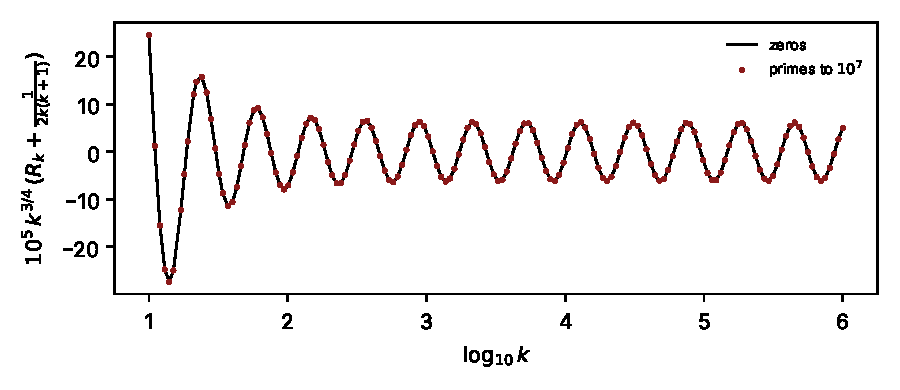
\includegraphics[width=0.8\textwidth]{fig/v3/cw_maslanka.pdf}
\caption{$k^{3/4}\big(R_k+\frac{1}{2k(k+1)}\big)$: primes (dots) and zeros (line). To leading order, under RH, this is $-\Re\,\Gamma(\frac34-\frac{i\gamma_1}2)k^{i\gamma_1/2}$, of amplitude $6.17\times10^{-5}$ and period $4\pi/\gamma_1=0.889$ in $\log k$ (computed).}
\label{cw:fig:maslanka}
\end{figure}

The theorem is the Williamson companion of Theorem~\ref{ct:thm:budget}. There the kernel is $2\sin^2$, the answer is a Thorin density, and the trivial zeros supply the allowance $G_\alpha$. Here the kernel is $(1-x^{-2})^k$, the sequence $d_k$ is positive for free, the trivial zeros contribute exactly $-1/(2k(k+1))$, and RH is a rate of decay. The input data are the values of $-\zeta'/\zeta$ at $2,4,6,\dots$, all at points to the right of the proved rungs; (ii) is a Newton interpolation from those rungs into the strip, an alternative to Cauchy deconvolution.

\begin{remark}\label{cw:rem:maslanka}
Does it help? It gives a positive measure where B\'aez-Duarte has a signed one, an exact formula and a sharp prime side test (Table~\ref{cw:tab:maslanka}). It does not give a path. Complete monotonicity of $(d_k)$ holds for every Beurling system, the rate $k^{-3/4}$ is carried by the zeros alone, and Newton interpolation no more preserves positivity than deconvolution does. The amplitude $|\Gamma(\frac34-\frac{i\gamma_1}{2})|=6.17\times10^{-5}$ explains why the oscillations in such criteria are hard to see numerically. We have not found the theorem in the literature, but a literature check for analogues of B\'aez-Duarte's criterion for $\zeta'/\zeta$ has not been made.
\end{remark}

\section{Williamson tilted Thorin densities}\label{cw:sec:williamson}

The factor $(1-n^{-2})^k$ is a positive reweighting of the L\'evy measure of $\zeta$: a Williamson tilt in place of the exponential tilt $n^{-\alpha}$. The $2\sin^2$ lemma applies to it unchanged. Let
\[
D_k(s)=\sum_n\frac{\Lambda(n)}{n^{s}}\Big(1-\frac1{n^2}\Big)^k,\qquad
Z_k(w)=\prod_{j=0}^k\zeta(2+2j+w)^{(-1)^j\binom kj},
\]
so that $D_k=-(\log Z_k)'$ at $s=2+w$ and $d_k=D_k(2)$.

\begin{proposition}[Williamson tilted Thorin densities]\label{cw:prop:williamson}
(a) For every $k\ge0$ the compensated reciprocal $\frac{Z_k(0)}{Z_k(w)}e^{-wD_k(2)}$ is a generalised gamma convolution in $u=w^2$, with Thorin density $T_k(\sqrt z)/(2\pi\sqrt z)$, where
\[
T_k(q)=D_k(2)-\Re D_k(2+iq)=\sum_n\frac{\Lambda(n)}{n^2}\Big(1-\frac1{n^2}\Big)^k\,2\sin^2\!\Big(\frac{q\log n}{2}\Big)\ \ge0 .
\]
(b) For $k\ge1$ and $\Re s>1$,
\[
D_k(s)=\tfrac12B\big(\tfrac{s-1}{2},k+1\big)-\tfrac12\sum_\rho B\big(\tfrac{s-\rho}{2},k+1\big)-\tfrac12\sum_{m\ge1}B\big(\tfrac s2+m,k+1\big).
\]
\end{proposition}

\begin{proof}
(a) With $\mu=\sum_n\Lambda(n)(n^2\log n)^{-1}(1-n^{-2})^k\delta_{\log n}\ge0$ the compensated reciprocal is $\exp\!\big(-\int(e^{-wx}+wx-1)\mu(\dd x)\big)$. Since $(1-e^{-wx})/w=\frac2\pi\int_0^\infty(1-\cos qx)(q^2+w^2)^{-1}\dd q$, the derivative of the exponent in $u=w^2$ is a Stieltjes transform, and integrating gives $\int\log(1+u/z)\,t(z)\,\dd z$ with $t(z)=(2\pi r)^{-1}\int x\,2\sin^2(rx/2)\,\mu(\dd x)$, $r=\sqrt z$, which is $T_k(r)/(2\pi r)$. (b) is the contour argument of Theorem~\ref{cw:thm:maslanka}(iii) with $-\frac{\zeta'}{\zeta}(s-2z)$ in place of $-\frac{\zeta'}{\zeta}(2-2z)$.
\end{proof}

For $k\ge1$ a zero contributes the Beta kernel $B(z,k+1)=k!/(z(z+1)\cdots(z+k))$ with $z=\frac12(2+iq-\rho)$, which decays like $|q-\gamma|^{-(k+1)}$, and $k^{z}B(z,k+1)\to\Gamma(z)$ pointwise. The Williamson order therefore sharpens the spectral window through which the primes see the zeros, from Cauchy at $k=0$ towards a Gamma function window as $k\to\infty$ (Figure~\ref{cw:fig:sin2}). At $k=0$ the Beta kernel is $B(z,1)=1/z$ and (b) is the partial fraction expansion behind Theorem~\ref{thm:poisson}, but the arcs of the contour do not vanish there, and the sum over the trivial zeros diverges, so (b) is stated for $k\ge1$ only (at $k=0$ it holds after regularisation). The weight also removes the integers below about $\sqrt k$: it is a smooth sieve acting on the Thorin measure.

\begin{table}[t]
\centering\small
\begin{tabular}{rrrr}
\toprule
$k$ & $q$ & $T_k(q)$ from primes & from (b), $400$ zeros\\
\midrule
$5$ & $3.0$ & $0.4030813914$ & $0.4030813914$\\
$20$ & $10.0$ & $0.1996901903$ & $0.1996901903$\\
$50$ & $14.1$ & $0.1566716107$ & $0.1566716107$\\
$200$ & $21.0$ & $0.0737517514$ & $0.0737517515$\\
\bottomrule
\end{tabular}
\caption{The two sides of Proposition~\ref{cw:prop:williamson} (computed). Prime powers up to $10^7$ with the tail added; the zero side adds the trivial zeros.}
\label{cw:tab:williamson}
\end{table}

\begin{figure}[t]
\centering
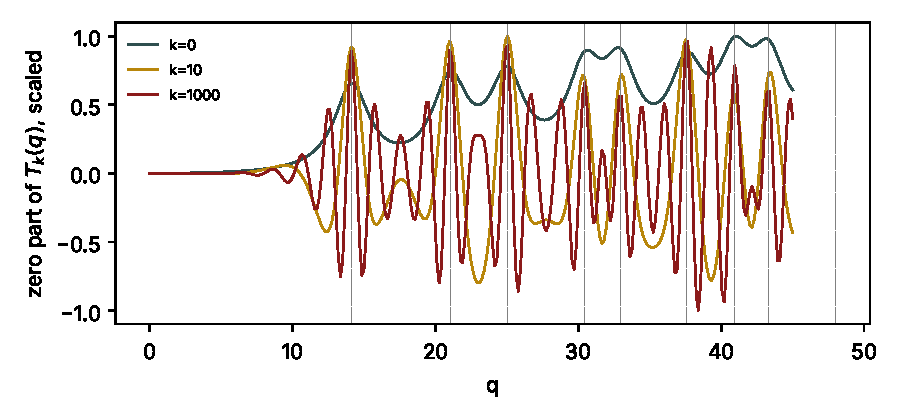
\includegraphics[width=0.8\textwidth]{fig/v3/cw_maslanka_sin2.pdf}
\caption{The contribution of the nontrivial zeros to $T_k(q)$, scaled to unit maximum, for $k=0,10,1000$. Peaks sit at the ordinates for every $k$. At $k=0$ the Cauchy tails overlap. For larger $k$ the peaks separate, at the price of negative side lobes.}
\label{cw:fig:sin2}
\end{figure}

\begin{remark}\label{cw:rem:williamson}
Two limits on what this gives. First, for $k\ge1$ the Beta kernel is not positive: its real part changes sign, as the side lobes in Figure~\ref{cw:fig:sin2} show. The positivity of $T_k$ comes from the primes, and the pole term $\frac12[B(\frac12,k+1)-\Re B(\frac{1+iq}{2},k+1)]$ of order $k^{-1/2}$ dominates the zero terms, of order $k^{-3/4}$ under RH and $O(k^{-9/16})$ by the theorem of \cite{OAI26a}. Second, the family lives at level $2$, to the right of the strip, so it is unconditional for the same reason as rung one. Its use is as a better window. In the deconvolution ladder the Cauchy kernel is what makes the descent ill posed. Replacing it by a Beta kernel of order $k$ is a regularisation with an exact prime side.
\end{remark}

\section{The error law: plane rotators and exit times}\label{cw:sec:law}

On RH, simple zeros and linear independence the Chebyshev error has the law of $Z=-\sum_{\gamma>0}a_\gamma\cos\theta_\gamma$ with $\theta_\gamma=\gamma y-\arg\rho$, $a_\gamma=2/\sqrt{\frac14+\gamma^2}$ and independent uniform angles (Rubinstein and Sarnak \cite{RubinsteinSarnak94}). The sign and the phase $\arg\rho=\arctan2\gamma$ do not change the law of one term, but they matter for relations between ordinates (Proposition~\ref{cw:prop:relation}).

\begin{proposition}[hitting time duality]\label{cw:prop:hit}
Assume RH, simple zeros and linear independence. Let $\tau_\gamma$ be independent copies of the exit time of planar Brownian motion from the unit disc, and $C=\frac12\sum_{\gamma>0}a_\gamma^2\tau_\gamma$. Then for $w\ge0$
\[
\frac{1}{\E\,e^{wZ}}=\prod_{\gamma>0}\frac{1}{I_0(a_\gamma w)}=\E\,e^{-w^2C},
\]
$C$ is a generalised gamma convolution in the book's chart with Thorin atoms $j_m^2/a_\gamma^2=\frac{j_m^2}{4}\big(\gamma^2+\frac14\big)$, and $\E\,C=\frac12\mathrm{Var}\,Z=G(1)=0.023096$.
\end{proposition}

\begin{proof}
For the planar exit time $\E e^{-s\tau}=1/I_0(\sqrt{2s})$ and $\E\tau=\frac12$, and $I_0(x)=\prod_m(1+x^2/j_m^2)$. Here $\mathrm{Var}\,Z=\frac12\sum a_\gamma^2=2G(1)$ by Theorem~\ref{cw:thm:cov}.
\end{proof}

This is a corollary of the Wald couple in the row of Table~\ref{c:tab:wald} with the arcsine law, $I_0$ and the Bessel process of dimension two, and the row with point masses, $\cosh$ and the exit of $(-1,1)$ is its Rademacher companion; the exit time and the hyperbolic secant law are in Section~\ref{r:sec:vj}. Only the explicit atoms for the Wintner law $Z$ are new. Each $\cos\theta_\gamma$ is a single plane rotator spin and $I_0(a_\gamma u)$ is its partition function in a field $u$. It has only imaginary zeros, the Lee and Yang property proved for rotators by Dunlop and Newman \cite{DunlopNewman75}. So $Z$ is a free ferromagnet of rotators with fields fixed by the zeros (there are no pair couplings, and the imaginary zeros of a single $I_0(au)$ are elementary, the interacting case being the theorem cited). Replacing the uniform angles by Rademacher signs gives $\cosh$ in place of $I_0$, the symmetric Meixner characteristic function $1/\cosh$ and the P\'olya Gamma variable of Polson, Scott and Windle \cite{PSW13}, with the Meixner L\'evy density in the sense of Grigelionis \cite{Grigelionis99}. The Chebyshev error is the two dimensional member of the family whose one dimensional member is Meixner.

\begin{proposition}[a relation among the ordinates]\label{cw:prop:relation}
Assume RH and simple zeros, and suppose the ordinates satisfy a relation $\gamma_i+\gamma_j=\gamma_k$. Put $c=\arg\rho_i+\arg\rho_j-\arg\rho_k$. Then $0<\cos c<1$, and the triple contributes $-\frac32a_ia_ja_k\cos c<0$ to the third cumulant of the limiting law of the error; a relation $2\gamma_i=\gamma_k$ contributes $-\frac34a_i^2a_k\cos c'<0$ with $c'=2\arg\rho_i-\arg\rho_k$. Every term has the same sign, so they cannot cancel: one such relation makes the law skewed to the left, and $\E e^{uZ}$ is not even in $u$, so it is not the product $\prod_{\gamma>0}I_0(a_\gamma u)$ of Proposition~\ref{cw:prop:hit}. Skewness alone does not exclude a statement of Thorin type in $u^2$ for $u\ge0$: if $N$ is Poisson with mean one, $1/\E e^{u(1-N)}=\exp(-(e^{-u}+u-1))$ is a generalised gamma convolution in $u^2$ by the argument of Proposition~\ref{cw:prop:williamson}(a).
\end{proposition}

\begin{proof}
With $\theta_k=\theta_i+\theta_j+c$, $\E[\cos\theta_i\cos\theta_j\cos(\theta_i+\theta_j+c)]=\frac14\cos c$, and the triple appears with multiplicity six in $\E Z^3$; the sign is that of $Z=-\sum a_\gamma\cos\theta_\gamma$. For $2\gamma_i=\gamma_k$, $\E[\cos^2\theta_i\cos(2\theta_i+c')]=\frac14\cos c'$ with multiplicity three. For the sign of $\cos c$ write $\arg\rho=\arctan2\gamma=\frac\pi2-\varepsilon_\gamma$ with $\varepsilon_\gamma=\arctan\frac1{2\gamma}\in(0,\frac\pi2)$ decreasing in $\gamma$. Then $c=\frac\pi2-(\varepsilon_i+\varepsilon_j-\varepsilon_k)$, and $0<\varepsilon_i<\varepsilon_i+\varepsilon_j-\varepsilon_k<\varepsilon_i+\varepsilon_j<\pi$ because $\gamma_k>\gamma_j$. Hence $\cos c=\sin(\varepsilon_i+\varepsilon_j-\varepsilon_k)\in(0,1)$. In the same way $\cos c'=\sin(2\varepsilon_i-\varepsilon_k)>0$. These are the only relations among three positive ordinates that enter $\E Z^3$, since a signed sum $\pm\gamma_p\pm\gamma_q\pm\gamma_r=0$ of positive numbers has one of these two forms.
\end{proof}

For large ordinates $\cos c\approx\frac1{2\gamma_i}+\frac1{2\gamma_j}-\frac1{2\gamma_k}$ is small but strictly positive, so the skewness of a single relation is small but never zero; for $\gamma_i,\gamma_j\ge14$ it is below $0.072$. If no relation among three ordinates holds, the third cumulant vanishes; relations with four or more terms enter only higher cumulants, and if every relation has an even number of terms the law can stay symmetric, and the question becomes a Lee and Yang problem for the Haar measure on a subtorus, which we leave open. Second moments, and hence Theorem~\ref{cw:thm:cov}, are unaffected.

\section{Chebyshev's weights}\label{cw:sec:weights}

Additive positivity is free and multiplicative positivity is lost. Let $\Phi\ge0$ be a bounded step function of the Landau and Bober type, with $f(s)=\zeta(s)P(s)=s\int_1^\infty\Phi(y)y^{-s-1}\dd y$.

\begin{proposition}[Chebyshev's weights]\label{cw:prop:chebw}
(a) For every $\alpha>0$ the function
\[
g_\alpha(w)=\frac{f(\alpha+w)}{\alpha+w}-\frac{f(\alpha)}{\alpha}-w\Big(\frac{f(s)}{s}\Big)'_{s=\alpha}
=\int_0^\infty\big(e^{-wx}+wx-1\big)e^{-\alpha x}\Phi(e^x)\,\dd x
\]
is of the form $\int\log(1+u/z)\,T(z)\,\dd z$ with $T\ge0$ and $u=w^2$, so $e^{-g_\alpha}$ is a generalised gamma convolution.

(b) For Chebyshev's $P(s)=1-2^{-s}-3^{-s}-5^{-s}+30^{-s}$ the function $f$ has no zero in $\Re s>1$, and for every $\alpha>1$ the compensated reciprocal $\frac{f(\alpha)}{f(\alpha+w)}e^{wf'(\alpha)/f(\alpha)}$ tends to $+\infty$ as $w\to+\infty$. So it is not a generalised gamma convolution, and the criterion $\Re\frac{f'}{f}(\alpha+iq)\ge\frac{f'}{f}(\alpha)$ fails at every level $\alpha>1$.
\end{proposition}

\begin{proof}
(a) This is the argument of Proposition~\ref{cw:prop:williamson}(a) with $\mu(\dd x)=e^{-\alpha x}\Phi(e^x)\dd x$ in place of the tilted prime measure, and it holds for every family in Bober's classification with no computation. (b) Put $a=2^{-\sigma}$, $b=3^{-\sigma}$, $c=5^{-\sigma}$ and $\theta_p=t\log p$. Since $1-\cos(\theta_2+\theta_3+\theta_5)\le3\sum_p(1-\cos\theta_p)$, $\Re P(\sigma+it)\ge P(\sigma)+\sum_p(p^{-\sigma}-3abc)(1-\cos\theta_p)\ge P(\sigma)$, and $P(\sigma)>0$ for $\sigma>1$ because $P(1)=0$ and $P'(\sigma)=(a-abc)\log2+(b-abc)\log3+(c-abc)\log5>0$; $\zeta$ has no zero there. Chebyshev's $\Phi$ takes the values $0$ and $1$, equals $1$ on $[1,6)$ and vanishes on intervals $[A_\ell,B_\ell)$ with $A_\ell\ge6$, so $f(\alpha)=1-\sum_\ell(A_\ell^{-\alpha}-B_\ell^{-\alpha})\in(0,1)$ and $f'(\alpha)=\sum_\ell(A_\ell^{-\alpha}\log A_\ell-B_\ell^{-\alpha}\log B_\ell)>0$, as $x^{-\alpha}\log x$ decreases for $x\ge6$. Since $f(\alpha+w)\to1$, the compensated reciprocal grows like $f(\alpha)e^{wf'(\alpha)/f(\alpha)}$, while a Laplace transform of a probability law is at most $1$.
\end{proof}

Table~\ref{cw:tab:chebw} shows where the criterion fails (computed):

\begin{table}[t]
\centering\small
\begin{tabular}{rrrr}
\toprule
$\alpha$ & $f'/f(\alpha)$ & $\min_{q\le200}$ of the difference & at $q$\\
\midrule
1.10 & 0.12812 & $-1.2798$ & 171.02\\
1.50 & 0.058942 & $-0.5330$ & 109.99\\
2.00 & 0.023294 & $-0.1812$ & 110.08\\
3.00 & 0.0039511 & $-0.0223$ & 110.17\\
\bottomrule
\end{tabular}
\caption{Failure of the criterion for Chebyshev's weights (computed). The difference is $\Re\frac{f'}{f}(\alpha+iq)-\frac{f'}{f}(\alpha)$.}
\label{cw:tab:chebw}
\end{table}

The prime term of $\zeta$ is nonnegative at every $q$, but $\log P$ has a signed L\'evy measure and its contribution is not. So Chebyshev's device trades the pole of $\zeta$ for a loss of positivity at the level of logarithms. This is the Beurling barrier seen from inside. Additive (Laplace level) positivity is cheap and is what Chebyshev, Landau's integrality criterion and Bober's classification are about. Multiplicative (Thorin level) positivity is what RH needs, and for $\xi$ it is supplied by the Gamma factor and the functional equation, not by the weights. The Diamond and Erd\H{o}s weight sequences have the same defect at every finite length (heuristic).

\section{What is open}\label{cw:sec:wopen}

The rungs $\alpha>\frac78$ are proved (Section~\ref{cw:sec:known}), and with them the identities of Theorem~\ref{cw:thm:cov}(i) and the bound $R_k=O(k^{-9/16})$. Below $\frac78$ every statement in this chapter is conditional on RH or on a zero free region.

\begin{enumerate}
\item Find a nonnegative kernel and measure representing $v_\alpha-b_\alpha$ on the whole strip. Landau's theorem needs a positive object defined without reference to the zeros, and after the pole is removed the measure $\dd\Delta$ is signed.
\item A Salem type criterion with a positive kernel (Remark~\ref{cw:rem:logistic}).
\item Even relations among the ordinates: is the Haar measure on the corresponding subtorus of Lee and Yang type?
\item Is there a statistical statement, that the estimate of $t_\alpha$ from primes at a given bandwidth is nonnegative with a margin uniform in the sample size, that would be evidence of a different kind from zero counting?
\end{enumerate}
